使用matplotlib对处理后的数据进行可视化展示. 除了楼盘价格分布的散点图,
行政区楼盘的直方图之外, 还增加了\textbf{楼盘数量分布的饼图},
以更好的体现各行政区域楼盘数量分布的特征, 通过与其楼盘均价和总价的综合参考,
可以发现更多的有关信息.
具体图表内容如下:
\begin{itemize}
    \item 楼盘价格分布的散点图~\ref{fig:楼盘价格分布的散点图}.
    \item 各行政区楼盘均价的直方图~\ref{fig:各行政区楼盘均价的直方图}.
    \item 各行政区楼盘总价的直方图~\ref{fig:各行政区楼盘总价的直方图}.
    \item 楼盘数量分布的饼图~\ref{fig:楼盘数量分布的饼图}.
    \item
        各行政区楼盘均价和总价对比的直方图~\ref{fig:各行政区楼盘均价和总价对比的直方图}.
\end{itemize}

各图表展示如下:
\begin{figure}[ht!]
    \begin{center}
        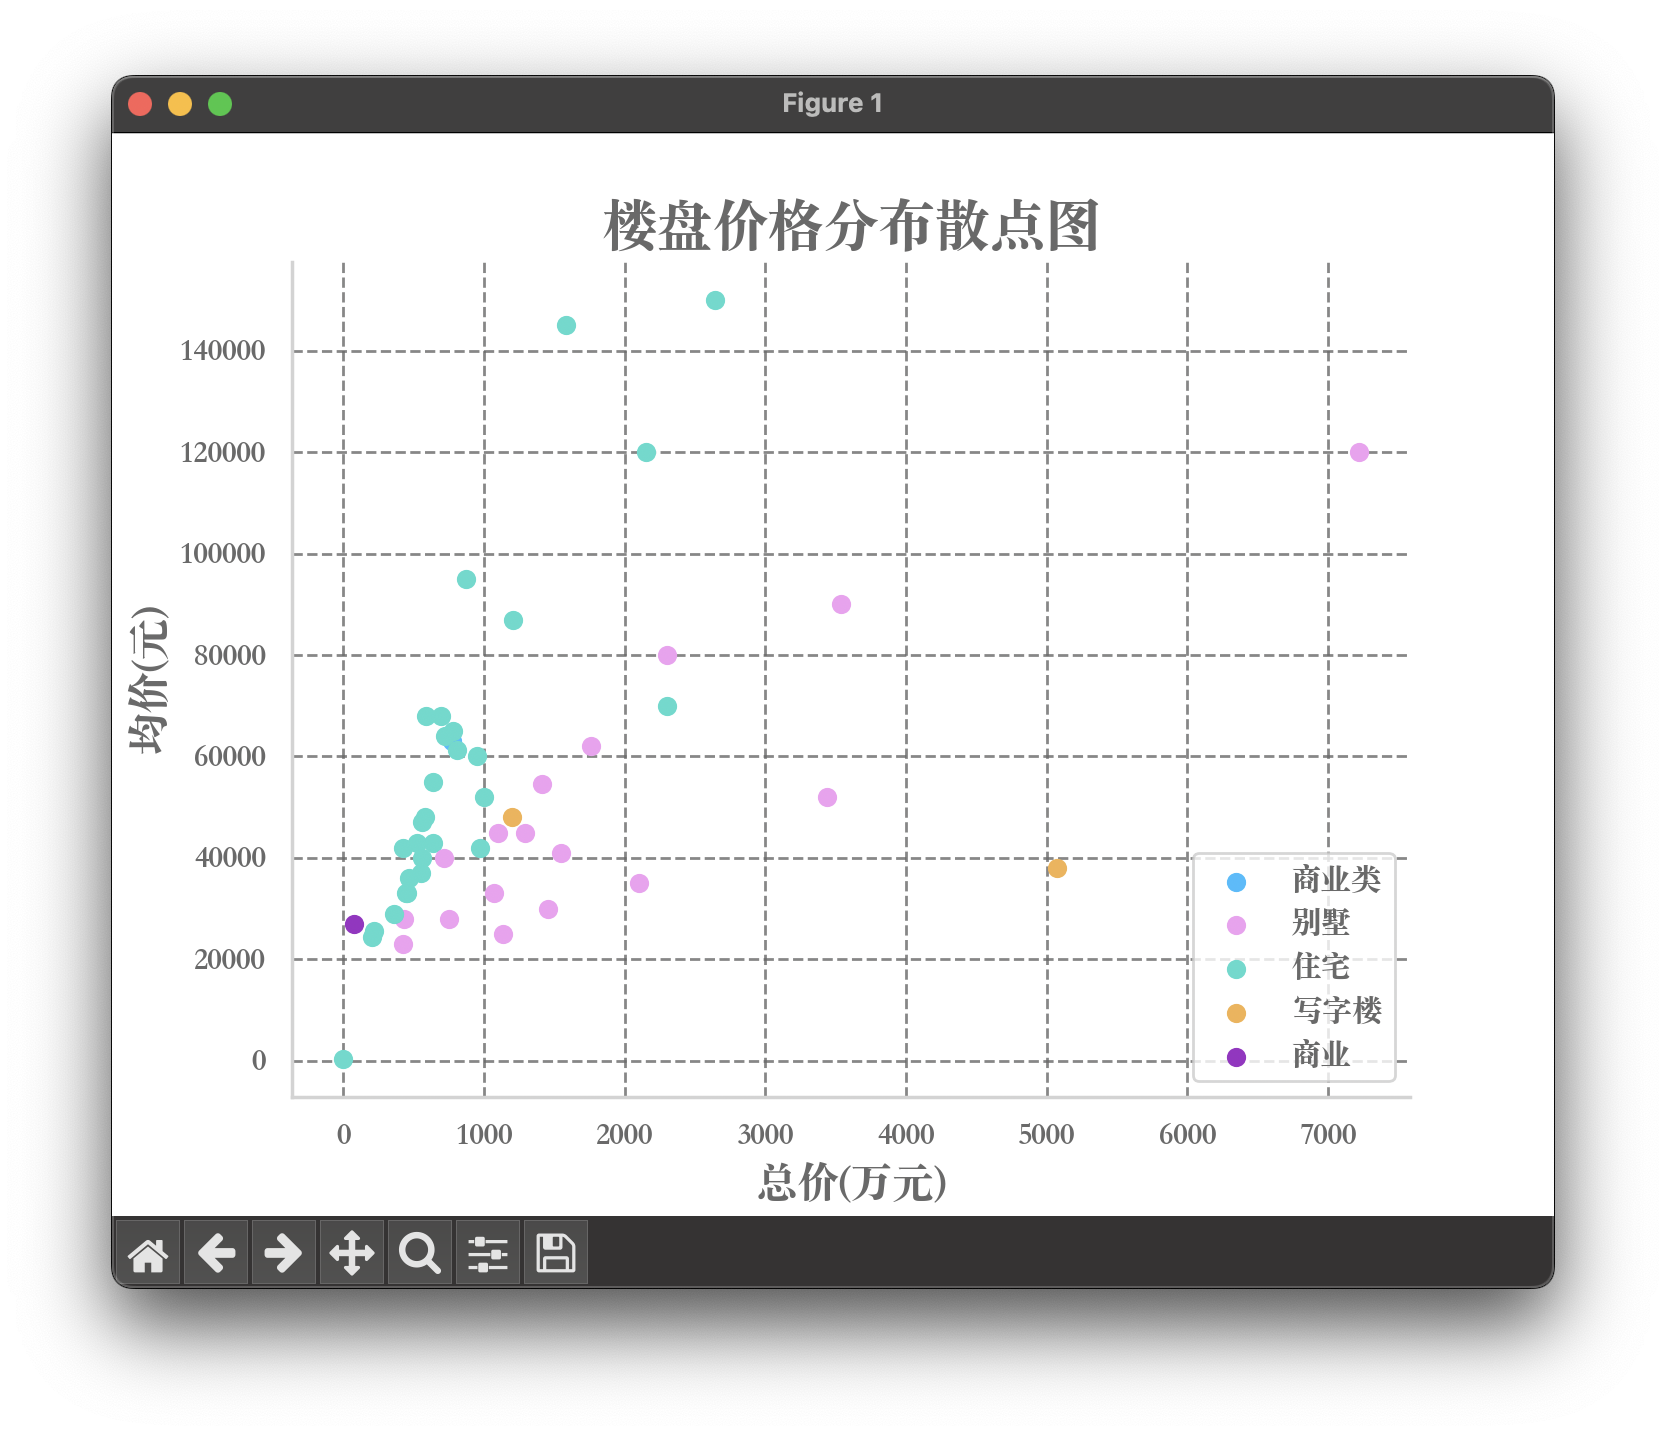
\includegraphics[width=0.95\textwidth]{figures/scatter.png}
    \end{center}
    \caption{楼盘价格分布的散点图}
    \label{fig:楼盘价格分布的散点图}
\end{figure}

\begin{figure}[ht!]
    \begin{center}
        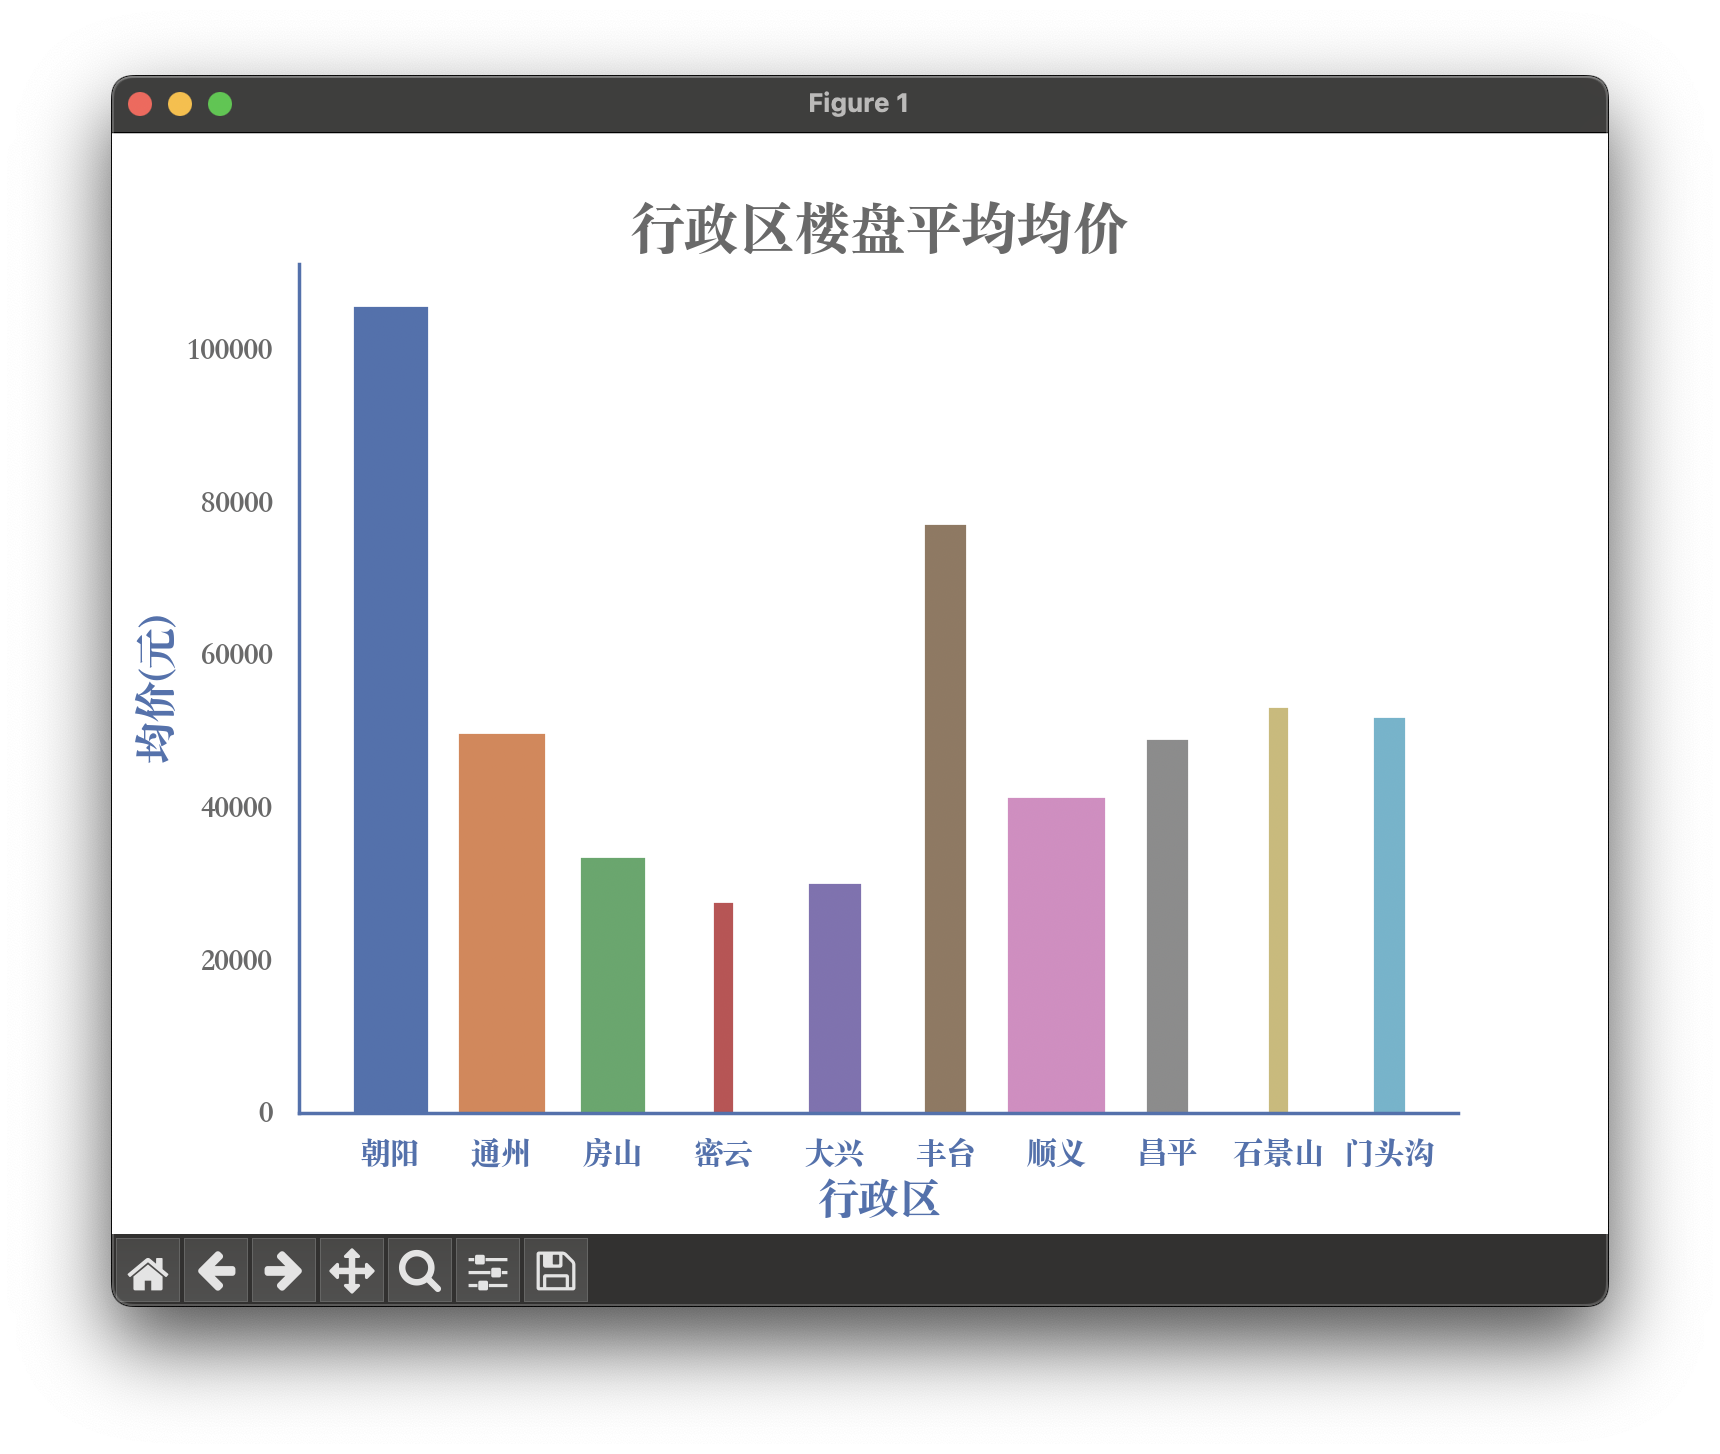
\includegraphics[width=0.95\textwidth]{figures/bar-avg.png}
    \end{center}
    \caption{各行政区楼盘均价的直方图}
    \label{fig:各行政区楼盘均价的直方图}
\end{figure}

\begin{figure}[ht!]
    \begin{center}
        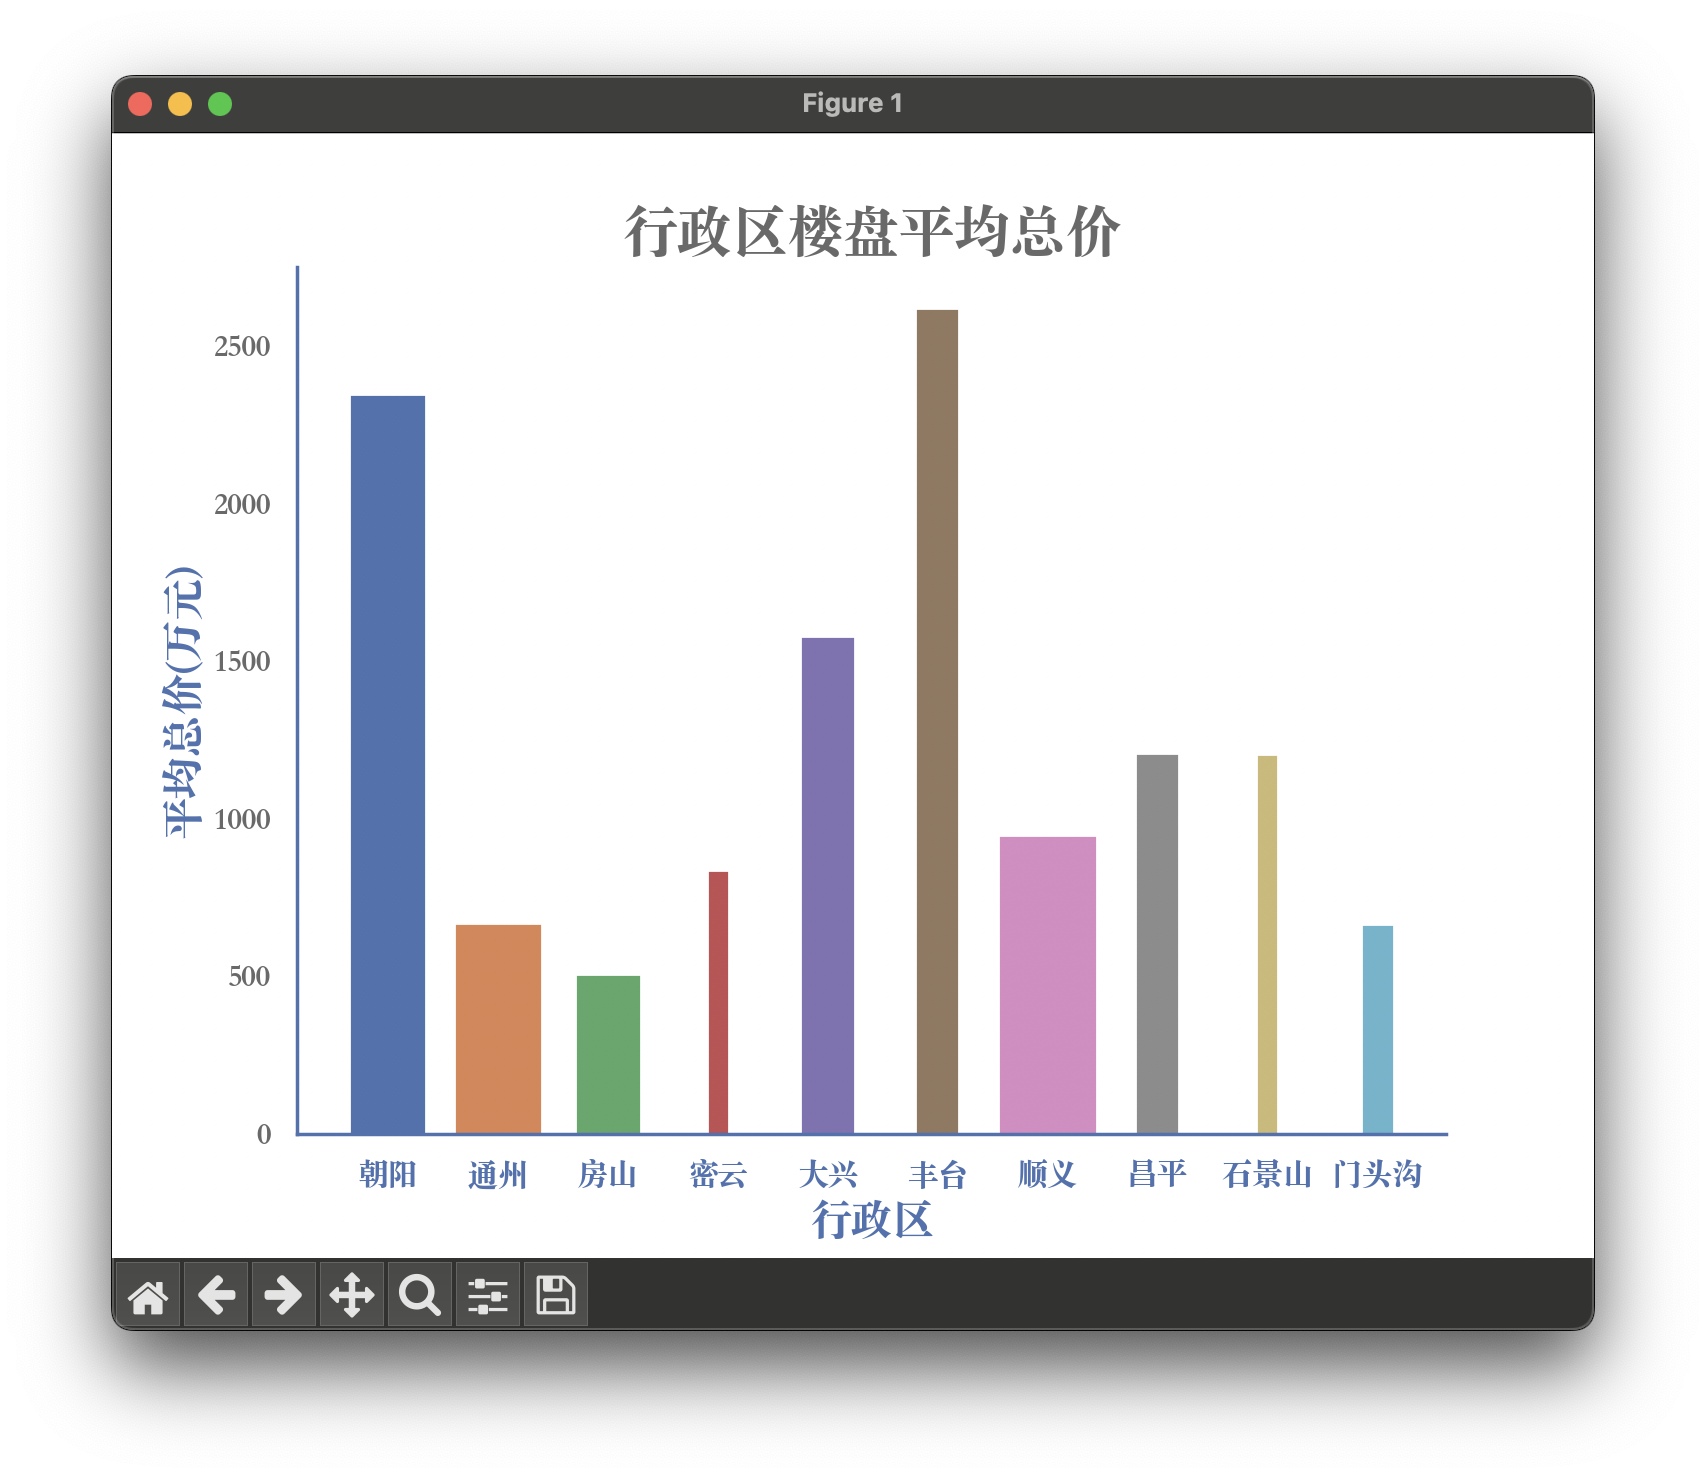
\includegraphics[width=0.95\textwidth]{figures/bar-total.png}
    \end{center}
    \caption{各行政区楼盘总价的直方图}
    \label{fig:各行政区楼盘总价的直方图}
\end{figure}

\begin{figure}[ht!]
    \begin{center}
        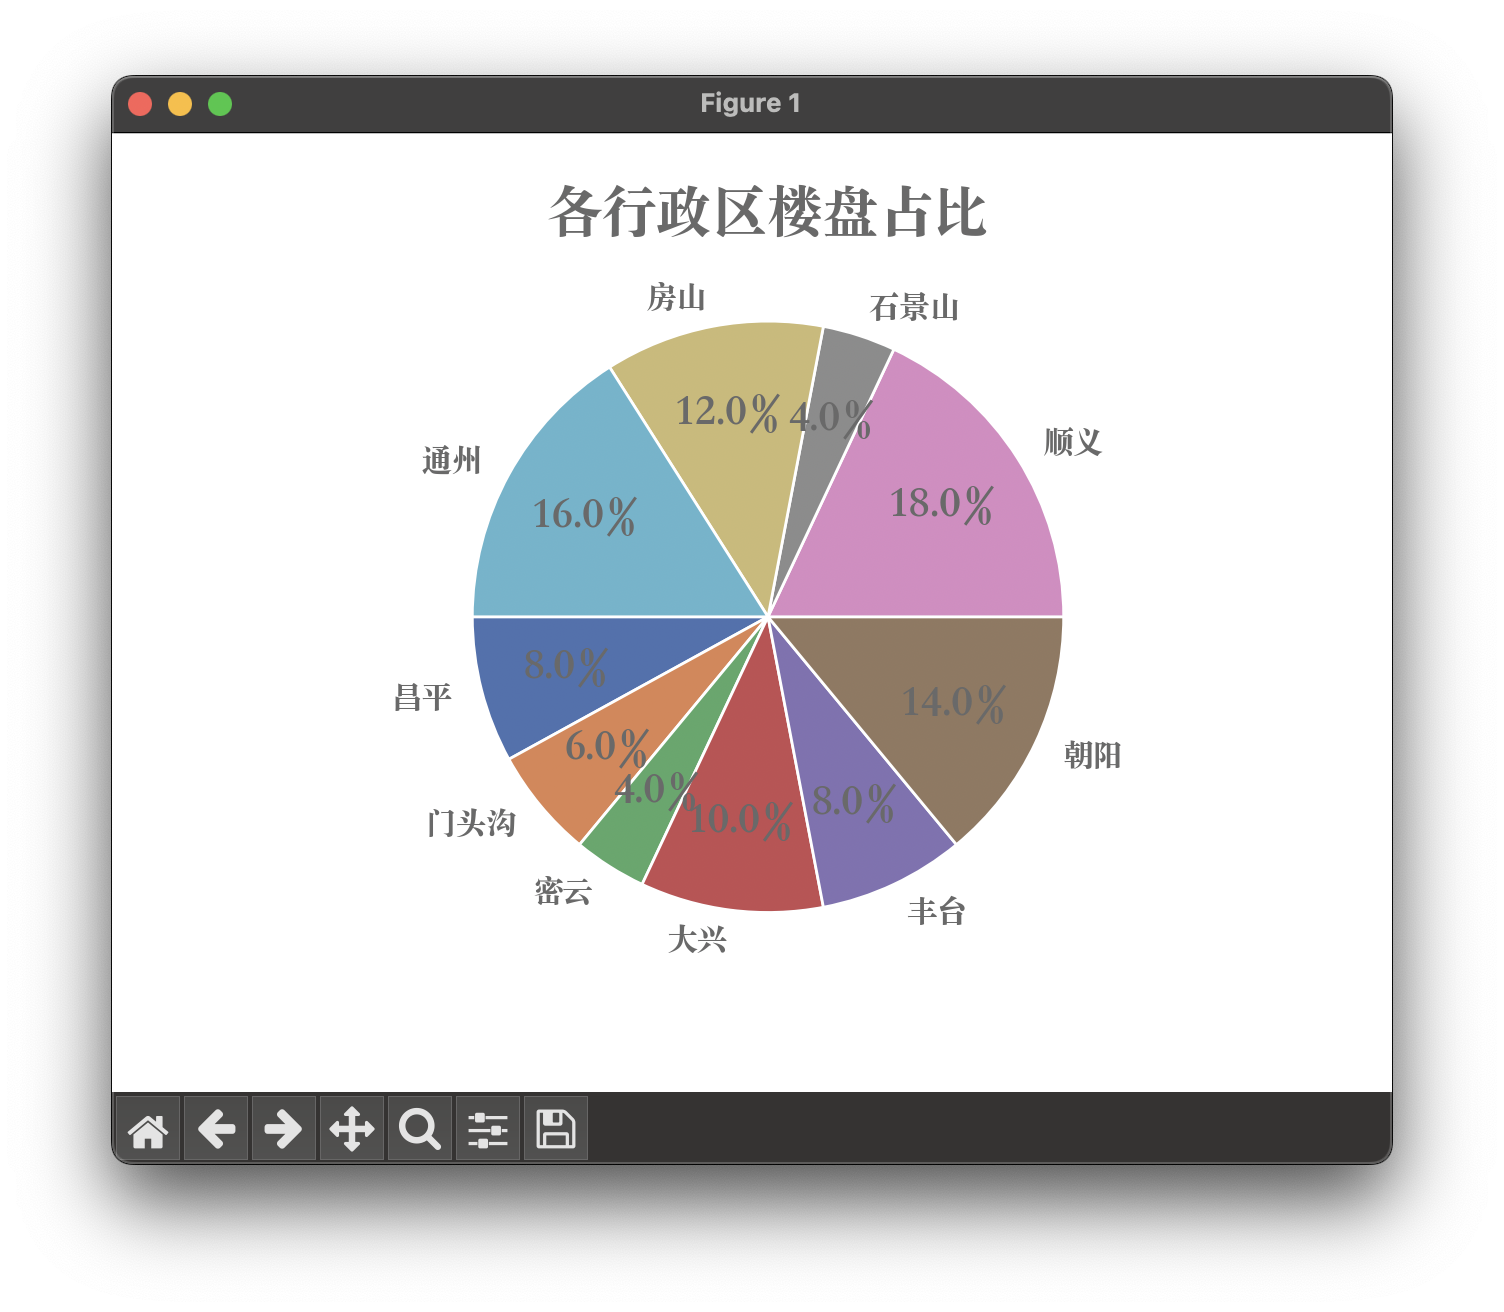
\includegraphics[width=0.95\textwidth]{figures/pie.png}
    \end{center}
    \caption{楼盘数量分布的饼图}
    \label{fig:楼盘数量分布的饼图}
\end{figure}

\begin{figure}[ht!]
    \begin{center}
        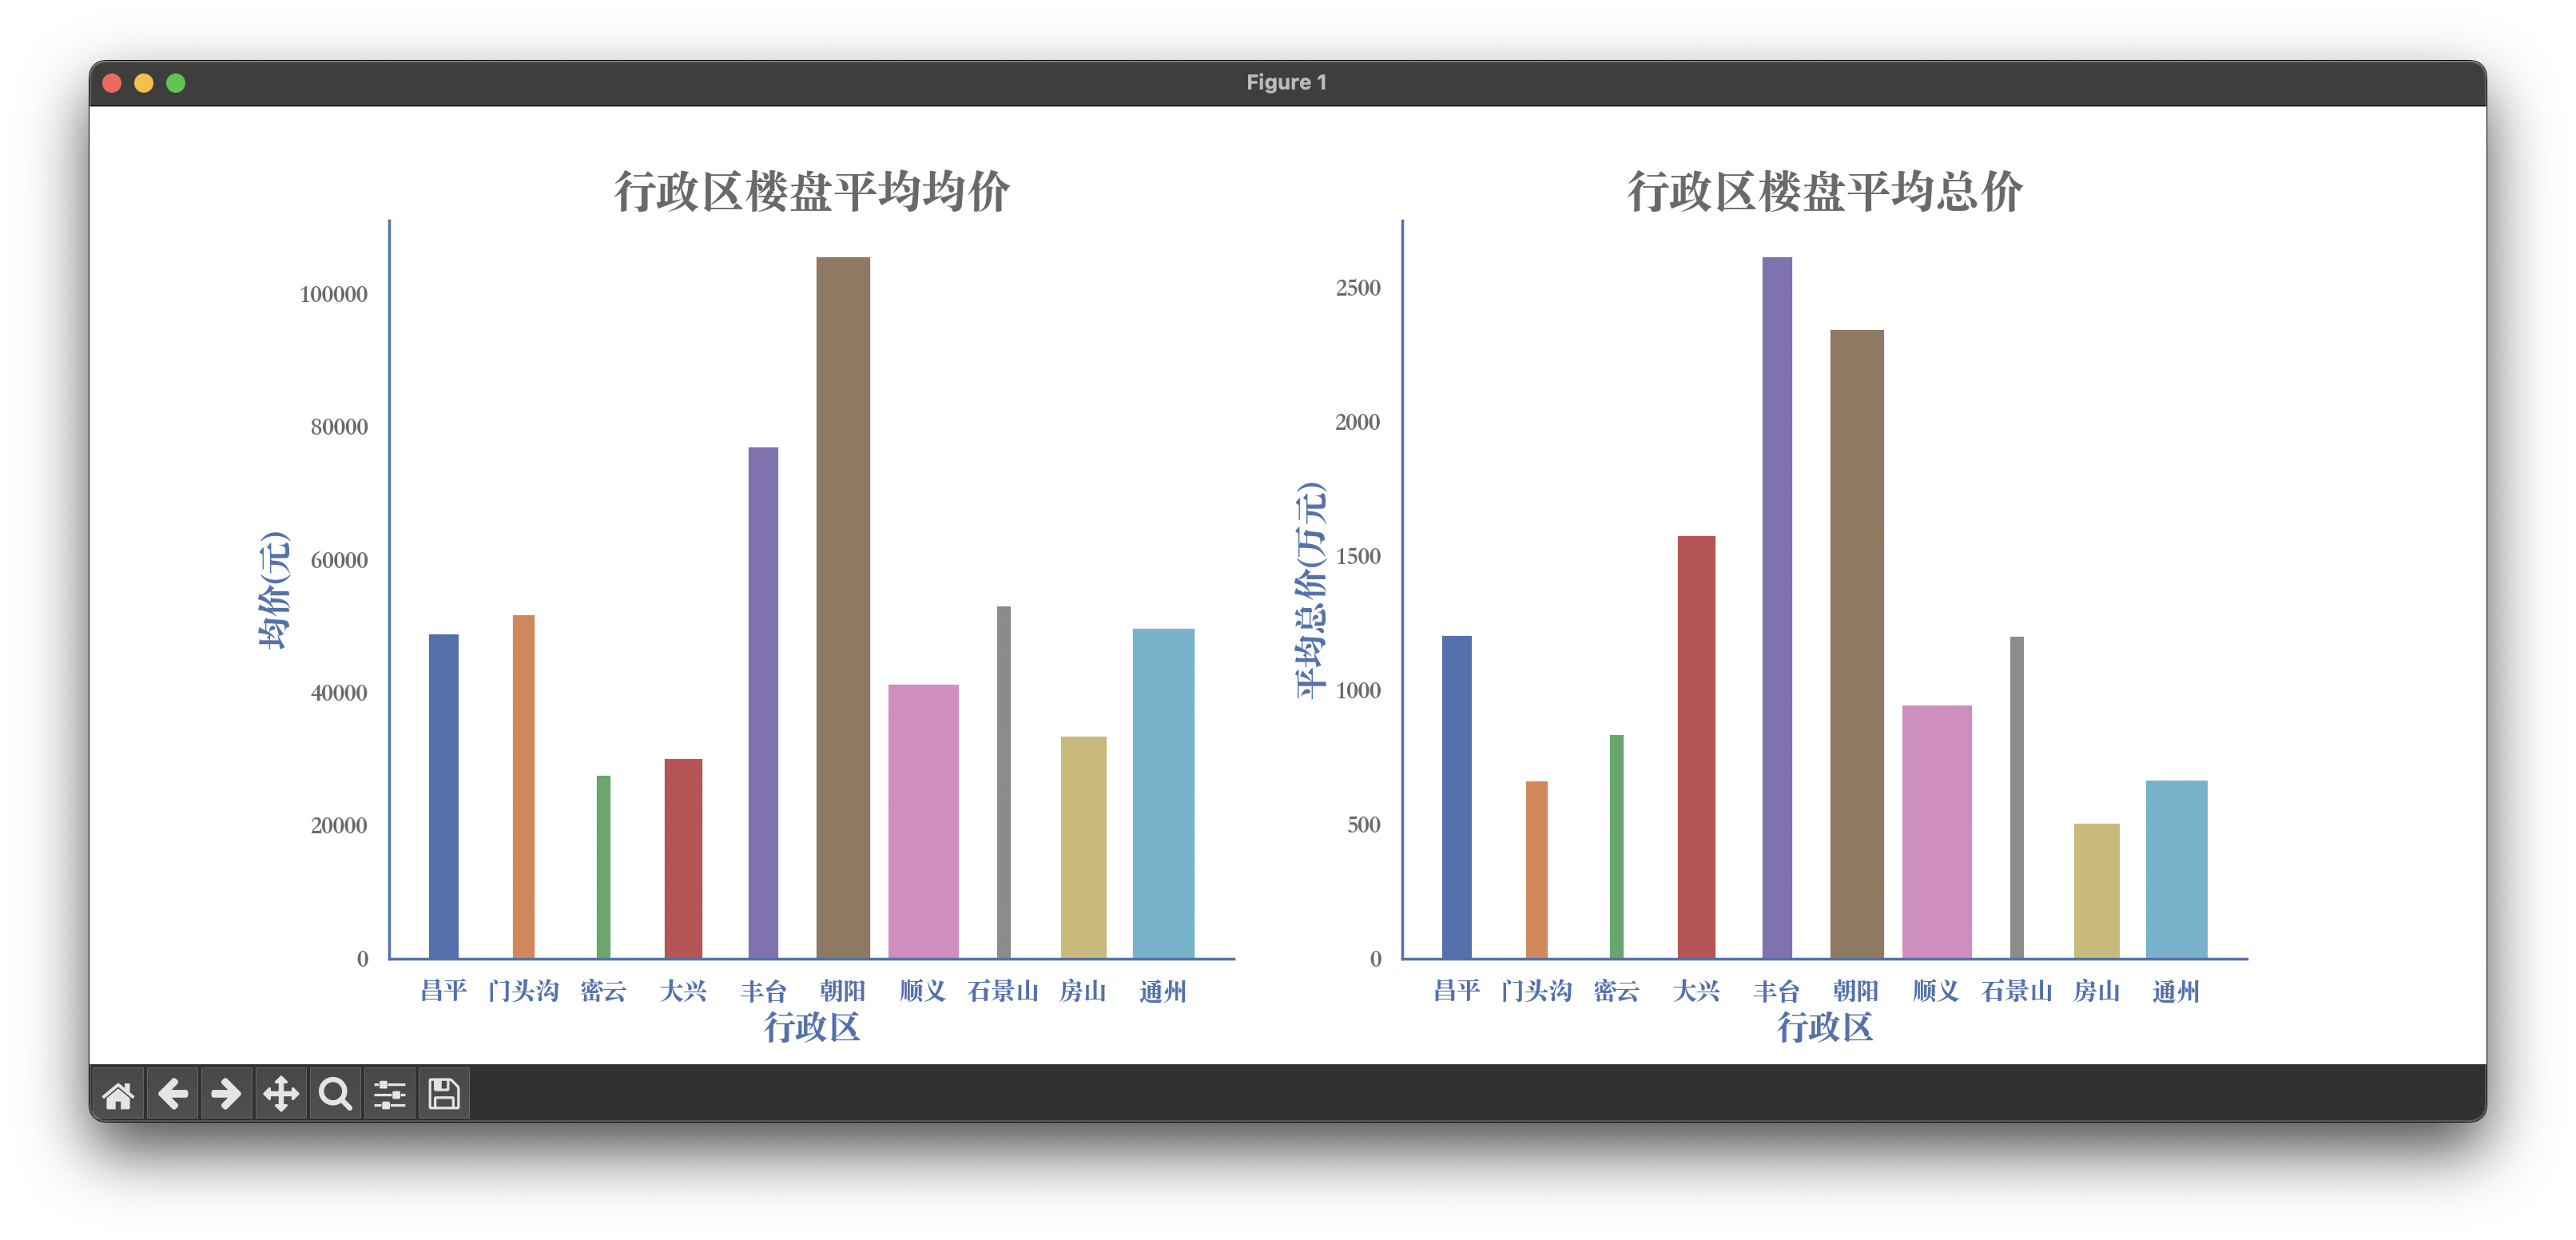
\includegraphics[width=0.95\textwidth]{figures/compare-bar.png}
    \end{center}
    \caption{各行政区楼盘均价和总价对比的直方图}
    \label{fig:各行政区楼盘均价和总价对比的直方图}
\end{figure}

